% This is part of Mes notes de mathématique
% Copyright (c) 2011-2016
%   Laurent Claessens
% See the file fdl-1.3.txt for copying conditions.

%+++++++++++++++++++++++++++++++++++++++++++++++++++++++++++++++++++++++++++++++++++++++++++++++++++++++++++++++++++++++++++
\section{Généralités}
%+++++++++++++++++++++++++++++++++++++++++++++++++++++++++++++++++++++++++++++++++++++++++++++++++++++++++++++++++++++++++++

La physique, et les sciences en général, regorge de fonctions à plusieurs variables.
\begin{description}
    \item[Accélération centripète]\footnote{Appelez la «centrifuge» si vous voulez; ça ne me fait ni chaud ni froid.}  Si une masse $m$ tourne sur un cercle, elle subira une accélération dirigée vers l'intérieur égale à
        \begin{equation}
            F(v,r)=\frac{ mv^2 }{ r }
        \end{equation}
        où $r$ est le rayon du cercle et $v$ est la vitesse.
    \item[Pression dans un gaz] Si on a $n$ moles de gaz dans un volume $V$ a une température $T$, alors la pression sera donnée par la fonction de trois variables
        \begin{equation}
            p=\frac{ nRT }{ V }
        \end{equation}
        où $R$ est la constante des gaz parfaits.
\end{description}
En mathématique, on peut inventer de nombreuses fonctions de plusieurs variables. La fonction
\begin{equation}
    f(x,y)=x^2+xy\cos(x^2+y^3)
\end{equation}
est définie sur $\eR^2$. La fonction
\begin{equation}
    f(x,y,z)=\frac{ x+y-2z }{ 1-x^2-y^2-z^2 }
\end{equation}
est définie sur $\eR^3$ moins la sphère unité $\{ x^2+y^2+z^2=1 \}$.

Le \defe{graphe}{graphe!fonction de deux variables} d'une fonction de deux variables $f\colon D\subset\eR^2\to \eR$ est l'ensemble
\begin{equation}
    \Big\{   \big( x,y,f(x,y) \big) \tq (x,y)\in D \Big\}\subset\eR^3.
\end{equation}
Ce graphe est une surface dans $\eR^3$.

\begin{example}     \label{ExempleTroisDxxyyOM}

    Tracer le graphe de la fonction 
    \begin{equation}
        (x,y)\mapsto x^2+y^2.
    \end{equation}
    Le plus simple est de demander à Sage de nous fournir une représentation 3D
    \begin{verbatim}
----------------------------------------------------------------------
| Sage Version 4.6.1, Release Date: 2011-01-11                       |
| Type notebook() for the GUI, and license() for information.        |
----------------------------------------------------------------------
sage: f(x,y)=x**2+y**2
sage: plot3d(f,(x,-3,3),(y,-3,3))
    \end{verbatim}
    
    Voici ce que cela donne\footnote{En vrai, ce que Sage donne est un objet qu'on peut même faire bouger.} : (à regarder avec des lunettes bleues et rouges) :
    \begin{center}
            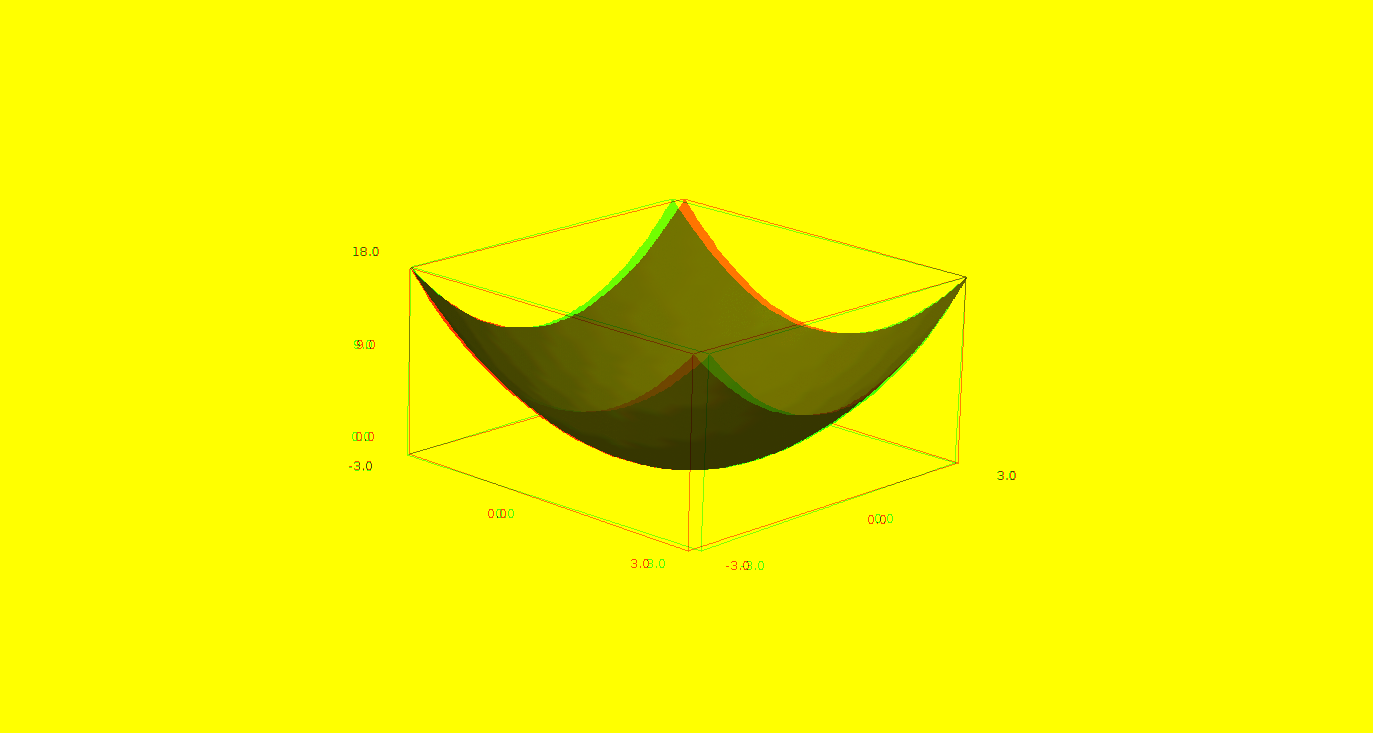
\includegraphics[width=15cm]{pictures_bitmap/coupe.png}
    \end{center}
    À part que l'ordinateur l'a dit, est-ce qu'on peut comprendre pourquoi le graphe de la fonction $x^2+y^2$ ressemble à un bol ? En coordonnées cylindriques, le graphe s'écrit
    \begin{equation}
        z=r^2.
    \end{equation}
    Donc il se fait que plus on s'éloigne du point $(0,0)$ dans le plan $XY$, plus le graphe va monter. Et il monte à quelle vitesse ? Il monte à la vitesse $r^2$. Il s'agit donc de dessiner la fonction $z=r^2$ dans le plan et de la «faire tourner».

\end{example}

%+++++++++++++++++++++++++++++++++++++++++++++++++++++++++++++++++++++++++++++++++++++++++++++++++++++++++++++++++++++++++++
\section{Courbes de niveau}
%+++++++++++++++++++++++++++++++++++++++++++++++++++++++++++++++++++++++++++++++++++++++++++++++++++++++++++++++++++++++++++

Une technique utile pour se faire une idée de la forme d'une fonction en trois dimensions est de tracer les \defe{courbes de niveau}{courbe de niveau}. La courbe de niveau de hauteur $h$ est la courbe dans le plan donnée par l'équation
\begin{equation}
    f(x,y)=h.
\end{equation}

\begin{example}

    Dessinons par exemple les courbes de niveau de la fonction
    \begin{equation}
        f(x,y)=x+y+2.
    \end{equation}
    La courbe de niveau $h$ est donnée par l'équation $x+y+2=h$, c'est à dire
    \begin{equation}
        y(x)=-x+h-2.
    \end{equation}
    Par conséquent la courbe de niveau de hauteur $0$ est $y=-x-2$, celle de hauteur $5$ est $y=-x+3$, etc.
    
    Nous pouvons également nous aider de Sage pour ce faire :
    \begin{verbatim}
----------------------------------------------------------------------
| Sage Version 4.6.1, Release Date: 2011-01-11                       |
| Type notebook() for the GUI, and license() for information.        |
----------------------------------------------------------------------
sage: f(x,y)=x+y+2
sage: var('h')                   
h
sage: niveau(h,x)=solve(f(x,y)==h,y)[0].rhs()
sage: g1(x)=niveau(1,x)
sage: g1
x |--> -x - 1
    \end{verbatim}
    Ici la fonction \verb+g1+ est la courbe de niveau $1$. 

    Si on veut faire tracer une courbe de niveau, Sage peut le faire :
    \begin{verbatim}
        sage: implicit_plot(f(x,y)==1,(x,-3,3),(y,-4,4))
    \end{verbatim}
    Cela tracera la courbe de niveau $h=1$ dans la partie du plan $x\in\mathopen[ -3 , 3 \mathclose]$ et $y\in\mathopen[ -4,4 ,  \mathclose]$.
    
\end{example}

Il est bien entendu possible de créer automatiquement $50$ courbes de niveau et de demander de les tracer toutes sur le même graphe.
\VerbatimInput[tabsize=3]{courbeNiveau.py}

Le résultat est :

\begin{center}
        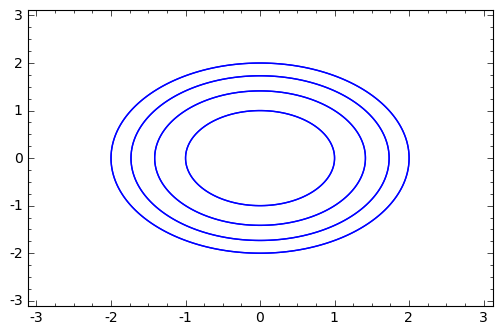
\includegraphics[width=8cm]{pictures_bitmap/niveauCercles.png}
\end{center}

\begin{example}
    Un exemple plus riche en enseignements est celui de la fonction
    \begin{equation}
        f(x,y)=x^2-y^2.
    \end{equation}
    La courbe de niveau $h$ est donnée par l'équation $x^2-y^2=h$.

    Commençons par $h=0$. Dans ce cas nous avons $(x+y)(x-y)=0$ et par conséquent les courbes de niveau de hauteur zéro sont les deux droites $x+y=0$ et $x-y=0$.

    Voyons ensuite la courbe de niveau $h=1$. Cela est l'équation $x^2-y^2=1$, c'est à dire
    \begin{equation}
        y(x)=\pm\sqrt{x^2-1}.
    \end{equation}
    C'est une fonction qui n'est définie que pour $| x |\geq 1$. Avec $x=1$ nous avons $y=1$. Ensuite, lorsque $x$ grandit, $y$ grandit également, mais la courbe ne peut pas croiser la courbe de niveau $h=0$. Donc, suivant les notations de la figure \ref{LabelFigNiveauHyperbole}, la courbe de niveau «part» de $P$ et doit monter sans croiser les diagonales.

    \newcommand{\CaptionFigNiveauHyperbole}{La courbe de niveau $h=1$ de $x^2-y^2$. Notez qu'elle est en deux morceaux.}
    \input{pictures_tex/Fig_NiveauHyperbole.pstricks}

    En ce qui concerne la courbe de niveau $h=-1$, elle correspond à la courbe $y=\pm\sqrt{1+x^2}$ qui est définie pour tous les $x\in\eR$. Le même raisonnement que précédemment nous amène à la figure \ref{LabelFigNiveauHyperboleDeux}.
\newcommand{\CaptionFigNiveauHyperboleDeux}{La courbe de niveau $x^2-y^2=-1$.}
\input{pictures_tex/Fig_NiveauHyperboleDeux.pstricks}


\end{example}

Une autre façon de voir les courbe de niveau est de dire que la courbe de niveau de hauteur $h$ est la projection dans le plan $XY$ de la section du graphe de $f$ par le plan $z=h$.

On peut également définir le graphe de fonctions de trois (ou plus) variables. Le graphe de la fonction $f\colon D\subset\eR^3\to \eR$ est l'ensemble
\begin{equation}
    \big\{ \big( x,y,z,f(x,y,z) \big)\tq (x,y,z)\in D \big\}\subset \eR^4.
\end{equation}
De tels graphes ne peuvent pas être représentés sur une feuille de papier. Il est toutefois possible de définir les ensembles de niveaux :
\begin{equation}
    E_h=\big\{ (x,y,z)\in D\tq  f(x,y,z)=h\big\}.
\end{equation}
Ce sont des surfaces dans $\eR^3$ que l'on peut dessiner.

\begin{example}
    Les surfaces de niveau de la fonction $f(x,y,z)=x^2+y^2+z^2$ sont des sphères. Il n'y a pas de surfaces de niveau pour les «hauteurs» négatives.
\end{example}

\begin{example}
    Considérons la fonction $f(x,y,z)=x^2+y^2-z^2$. En coordonnées cylindrique, cette fonction s'écrit
    \begin{equation}
        f(r,\theta,z)=r^2-z^2.
    \end{equation}
    La surface de niveau $0$ est donnée par l'équation $r=| z |$. Cela fait un cercle à chaque hauteur, dont le rayon grandit linéairement avec la hauteur; le tout est donc un cône. C'est d'ailleurs le cône obtenu par rotation de la courbe de niveau $h=0$ que nous avions obtenue pour la fonction $x^2-y^2$.

    En ce qui concerne les ensembles de niveau positifs, ils sont donnés par
    \begin{equation}
        z=\pm\sqrt{x^2+y^2-h}.
    \end{equation}
    Notez qu'ils ne sont pas définis pour $r\geq h$. Cela pose un petit problème quand on veut le tracer à l'ordinateur :
    \begin{verbatim}
----------------------------------------------------------------------
| Sage Version 4.6.1, Release Date: 2011-01-11                       |
| Type notebook() for the GUI, and license() for information.        |
----------------------------------------------------------------------
sage: var('x,y')
(x, y)
sage: f(x,y)=sqrt(x**2+y**2-3)
sage: F=plot3d(f(x,y),(x,-5,5),(y,-5,5)) 
sage: G=plot3d(-f(x,y),(x,-5,5),(y,-5,5))    
sage: F+G
    \end{verbatim}
Le résultat est\footnote{Encore une fois : ça donne mieux à l'écran, et vous pouvez le faire bouger; je vous encourage à le faire !} :
    \begin{center}
            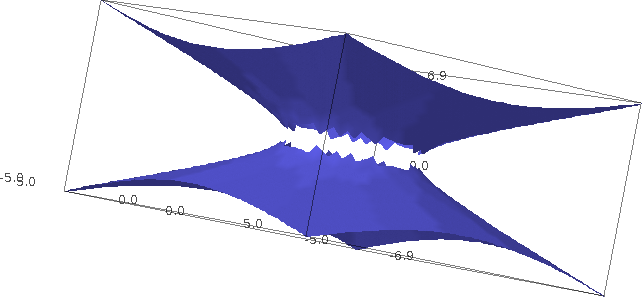
\includegraphics[width=15cm]{pictures_bitmap/AdSmauvais.png}
    \end{center}
    On voit qu'il y a un grand trou au centre correspondant aux $z$ proches de zéro. Or d'après l'équation, il n'en est rien : en $z=0$ il y a bel et bien tout un cercle. Afin d'obtenir une meilleur image, il faut demander de tracer avec un maillage plus fin :
    \begin{verbatim}
----------------------------------------------------------------------
| Sage Version 4.6.1, Release Date: 2011-01-11                       |
| Type notebook() for the GUI, and license() for information.        |
----------------------------------------------------------------------
sage: var('x,y')
(x, y)
sage: f(x,y)=sqrt(x**2+y**2-3)
sage: F=plot3d(f(x,y),(x,-5,5),(y,-5,5),plot_points=300) 
sage: G=plot3d(-f(x,y),(x,-5,5),(y,-5,5),plot_points=300)
sage: F+G
    \end{verbatim}
    Le temps de calcul est un peu plus long, mais le résultat est meilleur :
    \begin{center}
            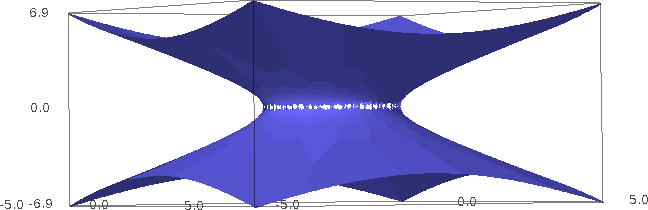
\includegraphics[width=15cm]{pictures_bitmap/AdSbon.png}
    \end{center}
\end{example}

%+++++++++++++++++++++++++++++++++++++++++++++++++++++++++++++++++++++++++++++++++++++++++++++++++++++++++++++++++++++++++++
\section{Dérivées partielles}
%+++++++++++++++++++++++++++++++++++++++++++++++++++++++++++++++++++++++++++++++++++++++++++++++++++++++++++++++++++++++++++

Soit $f\colon \eR^2\to \eR$ une fonction de deux variables et soit $(a,b)\in\eR^2$. La façon la plus naturelle de définir une dérivée à deux variables est de considérer les \defe{dérivées partielles}{dérivée!partielle} définies par
\begin{equation}
    \begin{aligned}[]
        \frac{ \partial f }{ \partial x }(a,b)&=\lim_{x\to a} \frac{ f(x,b)-f(a,b) }{ x-a }\\
        \frac{ \partial f }{ \partial y }(a,b)&=\lim_{y\to b} \frac{ f(a,y)-f(a,b) }{y-b}.
    \end{aligned}
\end{equation}
Ces nombres représentent la façon dont le nombre $f(x,y)$ varie lorsque soit seul $x$ varie soit seul $y$ varie. Les dérivées partielles se calculent de la même façon que les dérivées normales. Pour calculer $\partial_xf$, on fait «comme si» $y$ était une constante, et pour calculer $\partial_yf$, on fait comme si $x$ était une constante.

\begin{example}
    Considérons $f(x,y)=x^2y+y^2 e^{x}$. Les dérivées partielles sont
    \begin{equation}
        \begin{aligned}[]
            \frac{ \partial f }{ \partial x }&=2xy+y^2e^x\\
            \frac{ \partial f }{ \partial y }&=x^2+2ye^x.
        \end{aligned}
    \end{equation}
\end{example}

Cet exemple était l'exemple facile où tout se passe bien.

\begin{example}
    Les choses sont moins simples lorsqu'on considère la fonction suivante :
    \begin{equation}
        f(x,y)=\begin{cases}
            \frac{ xy }{ x^2+y^2 }    &   \text{si $(x,y)\neq(0,0)$}\\
            0    &    \text{si $(x,y)=(0,0)$}.
        \end{cases}
    \end{equation}
    On voit que pour tout $x$ et tout $y$, nous avons $f(x,0)=f(0,y)=0$. Donc cette fonction est nulle sur les axes horizontaux et verticaux. Nous avons en particulier
    \begin{equation}
        \begin{aligned}[]
            \frac{ \partial f }{ \partial x }(0,0)&=0\\
            \frac{ \partial f }{ \partial y }(0,0)&=0.
        \end{aligned}
    \end{equation}
    Donc ces dérivées partielles existe.

    Il n'est par contre pas question de dire que cette fonction «va bien» autour du point $(0,0)$. En effet si nous regardons sa valeur sur la droite diagonale $y=x$, nous avons
    \begin{equation}
        f(x,x)=\frac{ x^2 }{ 2x^2 }=\frac{ 1 }{2}.
    \end{equation}
    Par conséquent si nous suivons la fonction le long de la droite $y=x$, la hauteur vaut $\frac{ 1 }{2}$ en permanence, sauf juste en $(0,0)$ où la fonction fait un grand plongeon !
    \begin{verbatim}
    sage: var('x,y')
    (x, y)
    sage: f(x,y)=(x*y)/(x**2+y**2)
    sage: plot3d(f,(x,-2,2),y(-2,2))
    \end{verbatim}

    D'ailleurs elle fait un plongeon le long de toutes les droites (sauf verticale et horizontale). En effet si nous regardons la fonction le long de la droite $y=mx$, nous avons
    \begin{equation}
        f(x,mx)=\frac{ mx^2 }{ x^2+m^2x^2 }=\frac{ m }{ 1+m^2 }.
    \end{equation}
    La fonction est donc \emph{constante} sur chacune de ces droites. Il n'est donc pas question de dire que cette fonction est «dérivable» en $(0,0)$, vu qu'elle fait des grands sauts dans presque toutes les directions.
\end{example}

Nous devons donc trouver mieux que les dérivées partielles pour étudier le comportement des fonctions un peu problématiques.

Nous nous souvenons de l'équation \eqref{EqCodeDerviffxamOM} qui nous dit que pour une fonction d'une variable la dérivabilité signifiait qu'il existait un nombre $\ell$ et une fonction $\alpha$ tels
\begin{equation}
    f(x)=f(a)+\ell(x-a)+(x-a)\alpha(x-a)
\end{equation}
et $\lim_{t\to 0} \alpha(t)=0$. 

En nous inspirant de cela, nous posons la définition suivante.
\begin{definition}      \label{DefDiffabelOM}
    Une fonction $f\colon \eR^2\to \eR$ est \defe{différentiable}{différentiable} au point $(a,b)\in\eR^2$ s'il existe deux nombres $\ell_1$, $\ell_2$ ainsi qu'une fonction $\alpha$ tels que
    \begin{equation}\label{EqCondDiffabelOM}
        \begin{aligned}[]
            f(x,y)=f(a,b)&+\ell_1(x-a)+\ell_2(y-b)\\
                    &+\sqrt{(x-a)^2+(y-b)^2}\alpha\big( \sqrt{(x-a)^2+(y-b)^2} \big).
        \end{aligned}
    \end{equation}
\end{definition}

En utilisant la notation vectorielle, cela peut être écrite sous forme très compacte. Posons
\begin{equation}
    \begin{aligned}[]
        \ell&=\begin{pmatrix}
            \ell_1    \\ 
            \ell_2    
        \end{pmatrix},&
        X&=\begin{pmatrix}
            x    \\ 
            y    
        \end{pmatrix},&
        P&=\begin{pmatrix}
            a    \\ 
            b    
        \end{pmatrix}.
    \end{aligned}
\end{equation}
Alors la condition \eqref{EqCondDiffabelOM} s'écrit
\begin{equation}
    f(X)=f(P)+\ell\cdot(X-P)+\| X-P \|\alpha\big( \| X-P \| \big).
\end{equation}

\begin{proposition}
    Si $f$ est différentiable en $(a,b)$, alors les nombres $\partial_xf(a,b)$ et $\partial_yf(a,b)$ existent et valent respectivement $\ell_1$ et $\ell_2$.
\end{proposition}

\begin{proof}
    Afin de calculer la dérivée partielle dans la direction de $x$, nous posons $y=b$ dans la condition \eqref{EqCondDiffabelOM} :
    \begin{equation}
        f(x,b)=f(a,b)+\ell_1(x-a)+| x-a |\alpha\big( | x-a | \big),
    \end{equation}
    et donc
    \begin{equation}
        \frac{ f(x,b)-f(a,b) }{ x-a }=\ell_1\pm\alpha\big( | x-a | \big).
    \end{equation}
    Ici le $\pm$ est parce que nous avons divisé $(x-a)$ par $| x-a |$. Quel que soit ce signe, de toutes façons la limite du membre de droite lorsque $x$ tend vers $a$ est $\ell_1$ parce que $\lim_{x\to a} \alpha(| x-a |)=0$.

    Afin de prouver l'existence de la dérivée dans la direction de $y$, nous procédons de la même manière, mais en partant de $f(a,y)$.
\end{proof}

\begin{proposition}
    Si $f$ est différentiable au point $(a,b)$, alors elle y est continue, c'est à dire que
    \begin{equation}
        \lim_{(x,y)\to(a,b)}f(x,y)=f(a,b).
    \end{equation}
\end{proposition}

\begin{proof}
    Si nous considérons la différence entre $f(x,y)$ et $f(a,b)$, nous avons (en notations matricielle) :
    \begin{equation}
        | f(X)-f(P) |=| \ell\cdot(X-P)+\| X-P \|\alpha(\| X-P \|) |.
    \end{equation}
    Le membre de droite tend évidemment vers zéro lorsque $X$ tend vers $P$.
\end{proof}
    \begin{remark}
        Attention : ceci n'est pas une preuve. En effet, dans la mesure où nous n'avons même pas donné de définition de la limite, il n'est pas possible de donner une \emph{vraie} preuve de quoi que ce soit. 
    \end{remark}

Nous avons vu que l'existence des deux dérivées partielles ne permettait pas de conclure à la différentiabilité. La différentiabilité d'une fonction peut néanmoins être déduites d'une étude plus précise des dérivées partielles. Nous avons pour cela les propositions \ref{PropExistDiffUnOM} et \ref{PropExistDiffDeuxOM}

\begin{proposition} \label{PropExistDiffUnOM}
    Soit $f$ une fonction de $x$ et $y$ et un point $(a,b)\in\eR^2$. Si les nombres $\partial_xf(a,b)$ et $\partial_yf(a,b)$ existent et s'il existe une fonction $\alpha\colon \eR\to \eR$ telle que
    \begin{equation}        \label{eqCritDifffabsrtOM}
        \begin{aligned}[]
            f(x,y)=f(a,b)&+\frac{ \partial f }{ \partial x }(a,b)(x-a)+\frac{ \partial f }{ \partial y }(a,b)(y-b)\\
            &+\| (x,y)-(a,b) \| \alpha\Big( \| (x,y)-(a,b) \| \Big)
        \end{aligned}
    \end{equation}
    et
    \begin{equation}
        \lim_{t\to 0} \alpha(t)=0,
    \end{equation}
    alors $f$ est différentiable en $(a,b)$.
\end{proposition}
Dans cet énoncé nous avons écrit $d\big( (x,y),(a,b) \big)$ la distance entre $(x,y)$ et $(a,b)$, c'est à dire le nombre $\sqrt{(x-a)^2+(y-b)^2}$. Afin d'écrire l'équation \eqref{eqCritDifffabsrtOM} sous forme plus compacte, nous introduisons le vecteur
\begin{equation}
    \nabla f(a,b)=\begin{pmatrix}
        \frac{ \partial f }{ \partial x }(a,b)    \\ 
        \frac{ \partial f }{ \partial y }(a,b).    
    \end{pmatrix}
\end{equation}
L'équation \eqref{eqCritDifffabsrtOM} devient alors
\begin{equation}        \label{EqdiffCompOM}
    f(X)=f(P)+\nabla f(a,b)\cdot (X-P)+\| X-P \|\alpha\big( \| X-P \| \big).
\end{equation}
Le vecteur $\nabla f(a,b)$ est appelé le \defe{gradient}{gradient} de $f$ au point $(a,b)$.


\begin{proposition} \label{PropExistDiffDeuxOM}
    Soit $f$ une fonction de deux variables admettant des dérivées partielles $\partial_xf(x,y)$ et $\partial_yf(x,y)$ qui sont elles-mêmes des fonctions continues de $x$ et $y$. Alors la fonction $f$ est différentiable partout.
\end{proposition}

\begin{remark}
    Tout ce qui a été dit, et tout ce qui sera dit, sur les fonctions a deux variables se généralise immédiatement aux fonctions à plus de variables. C'est dans ce but que la notation «compacte» utilisant les vecteurs est très pratique.
\end{remark}

Si nous remplaçons les accroissements $x-a$ et $y-b$ par $h$ et $k$, le critère de différentiabilité s'écrit
\begin{equation}
    \begin{aligned}[]
        f(a+h,b+k)=f(a,b)+\frac{ \partial f }{ \partial x }(a,b)h&+\frac{ \partial f }{ \partial y }(a,b)k\\
        &+\sqrt{h^2+k^2}\alpha\big( \sqrt{h^2+k^2} \big).
    \end{aligned}
\end{equation}
Le dernier terme du membre de droite tend vers zéro à une vitesse double lorsque $h$ et $k$ tendent vers zéro : d'une part parce que $\sqrt{h^2+k^2}$ tend vers zéro et d'autre part parce que $\alpha\big( \sqrt{h^2+k^2} \big)$ tend vers zéro. Nous avons donc la «bonne» approximation
\begin{equation}        \label{EqFormApproxfxyabOM}
    f(x,y)\simeq f(a,b)+\frac{ \partial f }{ \partial x }(a,b)(x-a)+\frac{ \partial f }{ \partial y }(a,b)(y-b).
\end{equation}
lorsque $(x,y)$ n'est pas trop loin de $(a,b)$. Cette expression est évidemment une généralisation immédiate de l'équation \eqref{EqfxdxSimeqfxfpxOM}. Elle exprime que l'on peut obtenir des information sur la valeur d'une fonction en $(x,y)$ si on peut calculer la fonction et ses dérivées en un point $(a,b)$ non loin de $(x,y)$.

Cette formule peut aussi être vue sous la forme suivante, plus pratique dans certains calculs :
\begin{equation}        \label{EqFormApproxfxyabDFOM}
    f(a+\Delta x,b+\Delta y)\simeq f(a,b)+\Delta x\frac{ \partial f }{ \partial x }(a,b)+\Delta y\frac{ \partial f }{ \partial y }(a,b).
\end{equation}

\begin{example}
    Prenons la fonction $f(x,y)=\cos(x)\sin(y)$ et calculons une approximation de
    \begin{equation}
        f\big( \frac{ \pi }{ 3 }+0.01,\frac{ \pi }{ 2 }+0.03 \big).
    \end{equation}
    D'abord les dérivées partielles sont
    \begin{equation}
        \begin{aligned}[]
            \frac{ \partial f }{ \partial x }(x,y)=-\sin(x)\sin(y)\\
            \frac{ \partial f }{ \partial y }(x,y)=\cos(x)\cos(y).
        \end{aligned}
    \end{equation}
    Nous allons utiliser l'approximation
    \begin{equation}
        f\big( \frac{ \pi }{ 3 }+0.01,\frac{ \pi }{ 2 }+0.03 \big)\simeq f\big( \frac{ \pi }{ 3 },\frac{ \pi }{2} \big)+0.01\frac{ \partial f }{ \partial x }\big( \frac{ \pi }{ 3 },\frac{ \pi }{2} \big)+0.03\frac{ \partial f }{ \partial y }\big( \frac{ \pi }{ 3 },\frac{ \pi }{2} \big).
    \end{equation}
    Nous avons
    \begin{equation}
        \begin{aligned}[]
            \frac{ \partial f }{ \partial x }\big( \frac{ \pi }{ 3 },\frac{ \pi }{2} \big)&=-\sin\frac{ \pi }{ 3 }\sin\frac{ \pi }{ 2 }=-\frac{ \sqrt{3} }{2}\\
            \frac{ \partial f }{ \partial y }\big( \frac{ \pi }{ 3 },\frac{ \pi }{2} \big)&=\cos\frac{ \pi }{ 3 }\cos\frac{ \pi }{ 2 }=0.
        \end{aligned}
    \end{equation}
    Par conséquent
    \begin{equation}
        f\big( \frac{ \pi }{ 3 }+0.01,\frac{ \pi }{ 2 }+0.03 \big)\simeq \frac{ 1 }{2}-0.01\frac{ \sqrt{3} }{2}=\frac{ 1 }{2}-\frac{ \sqrt{3} }{ 200 }. 
    \end{equation}
    
    \begin{verbatim}
sage: var('x,y')
(x, y)
sage: f(x,y)=cos(x)*sin(y)
sage: a=f(pi/3+0.01,pi/2+0.03)
sage: numerical_approx(a)
0.491093815387986
sage: b=1/2-sqrt(3)/200
sage: numerical_approx(b)
0.491339745962156
sage: numerical_approx(a-b)
-0.000245930574169814
    \end{verbatim}
    Cela fait une erreur de l'ordre du dix millième. 
    
\end{example}

\begin{remark}
    Les esprits les plus critiques diront que cette vérification pas Sage n'en est pas une parce que Sage a certainement utilisé un algorithme d'approximation qui se base sur la même idée que ce que nous venons de faire, et que par conséquent le fait qu'il obtienne le même résultat que nous est un peu tautologique. 
    
    Ils n'auront pas tord. Cependant, le code source de Sage est disponible publiquement\footnote{Voir \url{http://www.sagemath.org}}; vous pouvez aller le lire et vérifier qu'il y a effectivement une \emph{preuve} que le résultat fourni par Sage possède une bonne dizaine de décimales correctes. 
    
    Cette disponibilité publique du code source est une des nombreuses différence fondamentale entre Sage et votre calculatrice\footnote{et les autres logiciels de type fenêtre, pomme ou feuille d'érable.}. Dois-je vous rappeler qu'un des principes fondamentaux de l'éthique scientifique est que les résultats et les méthodes utilisées doivent être absolument ouverts à la vérification et à la critique de tous ?
\end{remark}

%---------------------------------------------------------------------------------------------------------------------------
\subsection{Différentielle}
%---------------------------------------------------------------------------------------------------------------------------

\begin{definition}      \label{DefDiffrdrrOM}
    Lorsque $f$ est différentiable au point $(a,b)$, on appelle \defe{différentielle}{différentielle} de $f$ l'application linéaire
    \begin{equation}        \label{EqDefDiffmapdfOM}
        \begin{aligned}
            df_{(a,b)}\colon \eR^2&\to \eR \\
            \begin{pmatrix}
                u_1    \\ 
                u_2    
            \end{pmatrix}&\mapsto \frac{ \partial f }{ \partial x }(a,b)u_1+\frac{ \partial f }{ \partial y }(a,b)u_2. 
        \end{aligned}
    \end{equation}
    En notations compacte :
    \begin{equation}        \label{EqdfUPnableOM}
        df_{P}(U)=\nabla f(P)\cdot U.
    \end{equation}
\end{definition}

Note : dans la suite nous allons rendre notre «notation compacte» plus agréable à lire en abandonnant les majuscules. L'équation \eqref{EqdfUPnableOM} s'écrira donc
\begin{equation}        \label{EqdfpunfpduOM}
    df_p(u)=\nabla f(p)\cdot u.
\end{equation}


%+++++++++++++++++++++++++++++++++++++++++++++++++++++++++++++++++++++++++++++++++++++++++++++++++++++++++++++++++++++++++++
\section{Plan tangent au graphe d'une fonction}
%+++++++++++++++++++++++++++++++++++++++++++++++++++++++++++++++++++++++++++++++++++++++++++++++++++++++++++++++++++++++++++

Nous avons vu que, de la même façon qu'en deux dimensions nous avions l'approximation \eqref{EqfxsimesfaOM} d'une fonction par sa tangente, en trois dimensions nous avons l'approximation suivante d'une fonction de deux variables :
\begin{equation}
    f(x,y)\simeq f(a,b)+\frac{ \partial f }{ \partial x }(a,b)(x-a)+\frac{ \partial f }{ \partial y }(a,b)(y-b)
\end{equation}
lorsque $(x,y)$ n'est pas trop loin de $(a,b)$. Cela signifie que le graphe de $f$ ressemble au graphe de la fonction $T_{(a,b)}$ donnée par
\begin{equation}
    T_{(a,b)}(x,y)=f(a,b)+\frac{ \partial f }{ \partial x }(a,b)(x-a)+\frac{ \partial f }{ \partial y }(a,b)(x-a).
\end{equation}
En notations compactes :
\begin{equation}
    T_p(x)=f(p)+\nabla f(p)\cdot (x-p).
\end{equation}
Le graphe de la fonction $T_p$ sera le \defe{plan tangent}{plan!tangent} au graphe de $f$ au point $p$. L'équation du plan tangent sera donc
\begin{equation}
    z-f(p)=\nabla f(p)\cdot (x-p).
\end{equation}

\begin{remark}
    Lorsque nous utilisons la notation vectorielle, la lettre «$x$» désigne le vecteur $(x,y)$. Il faut être attentif. Dans un cas $x$ est un vecteur dans l'autre c'est une composante d'un vecteur.
\end{remark}




%+++++++++++++++++++++++++++++++++++++++++++++++++++++++++++++++++++++++++++++++++++++++++++++++++++++++++++++++++++++++++++
\section{Dérivée directionnelle}
%+++++++++++++++++++++++++++++++++++++++++++++++++++++++++++++++++++++++++++++++++++++++++++++++++++++++++++++++++++++++++++

Nous sommes capables de dériver une fonction de deux variables $f(x,y)$ par rapport à $x$ et par rapport à $y$. C'est à dire que nous sommes capables de donner la variation de la fonction lorsqu'on bouge le long des axes horizontal et vertical. Il est évidemment souhaitable de parler de la variation de la fonction lorsqu'on se déplace le long d'autre droites.

Soit donc $u=\begin{pmatrix}
    u_1    \\ 
    u_2    
\end{pmatrix}$ un vecteur unitaire (c'est à dire $u_1^2+u_2^2=1$), et considérons la fonction de une variable
\begin{equation}
    \begin{aligned}
        \varphi\colon \eR&\to \eR \\
        t&\mapsto f(a+tu_1,b+tu_2). 
    \end{aligned}
\end{equation}
La fonction $\varphi$ n'est rien d'autre que la fonction $f$ vue le long de la droite de direction donnée par le vecteur $u$. Nous pouvons aussi l'écrire $\varphi(t)=f(p+tu)$.

\begin{proposition}
    Si $f$ est différentiable en $(a,b)$ alors la fonction $\varphi$ est dérivable en $0$ et on a
    \begin{equation}
        \varphi'(0)=\nabla f(p)\cdot u
    \end{equation}
    où nous avons noté $p=(a,b)$.
\end{proposition}

\begin{proof}
    Récrivons la formule \eqref{EqdiffCompOM} sous la forme
    \begin{equation}
        f(x)=f(p)+\nabla f(p)\cdot (x-p)+\| x-p \|\alpha(\| x-p \|).
    \end{equation}
    Cela étant vrai pour tout $x$, nous l'écrivons en particulier pour $x=p+tu$ où $t$ est un réel et $u$ est le vecteur unitaire choisi. Nous avons donc
    \begin{equation}
        f(p+tu)=f(p)+t\nabla f(p)\cdot u+\| tu \|\alpha(\| tu \|).
    \end{equation}
    En utilisant le fait que $u$ est unitaire, $\| tu \|=| t |\| u \|=| t |$. La dérivée de $\varphi$ en $0$ est alors donnée par
    \begin{equation}
        \lim_{t\to 0} \frac{ f(p+tu)-f(p) }{ t }=\lim_{t\to 0} \nabla f(p)\cdot u+\alpha(| t |).    
    \end{equation}
    Lorsque nous prenons la limite, le membre de gauche devient $\varphi'(0)$ tandis que dans le membre de droite, le second terme disparaît. Nous avons finalement
    \begin{equation}
        \varphi'(0)=\nabla f(p)\cdot u
    \end{equation}
\end{proof}

\begin{definition}
    Le nombre
    \begin{equation}
        \lim_{t\to 0} \frac{ f\big( a+tu_1,b+tu_2 \big)-f(a,b) }{ t }
    \end{equation}
    est la \defe{dérivée directionnelle}{dérivée!directionnelle} de $f$ dans la direction de $u$ au point $(a,b)$. Il sera noté
    \begin{equation}
        \frac{ \partial f }{ \partial u }(a,b),
    \end{equation}
    ou plus simplement $\partial_uf(a,b)$.
\end{definition}

Lorsque $f$ est différentiable, la dérivée directionnelle est donnée par
\begin{equation}        \label{EqDerDirnablauOM}
    \frac{ \partial f }{ \partial u }(p)=\nabla f(p)\cdot u.
\end{equation}

En combinant avec l'équation \eqref{EqdfpunfpduOM}, nous avons la suite d'égalités
\begin{equation}        \label{EqsuitedfnfdsdfuOM}
    df_p(u)=\nabla f(p)\cdot u=\frac{ \partial f }{ \partial x }(p)u_1+\frac{ \partial f }{ \partial y }(p)u_2+\frac{ \partial f }{ \partial z }(p)u_3=\frac{ \partial f }{ \partial u }(p).
\end{equation}
La dernière équation est seulement vraie si $\| u \|=1$.

%---------------------------------------------------------------------------------------------------------------------------
\subsection{Gradient : direction de plus grande pente}
%---------------------------------------------------------------------------------------------------------------------------

Étant donné que $u$ est de norme $1$, l'inégalité de Cauchy-Schwartz donne
\begin{equation}
    \big| \nabla f(a,b)\cdot \begin{pmatrix}
        u_1    \\ 
        u_2    
    \end{pmatrix}\big|\leq \| \nabla f(a,b) \|.
\end{equation}
Donc
\begin{equation}
    -\| \nabla f(p) \|\leq \nabla f(p)\cdot u\leq\| \nabla f(p) \|.
\end{equation}
La norme de la dérivée directionnelle (qui est la valeur absolue du nombre au centre) est donc «coincée» entre $-\| \nabla f(p) \|$ et $\| \nabla f(p) \|$. Prenons par exemple
\begin{equation}
    u=\frac{ \nabla f(p) }{ \| \nabla f(p) \| }.
\end{equation}
Dans ce cas, nous avons exactement
\begin{equation}
    \nabla f(p)\cdot u=\| \nabla f(p) \|,
\end{equation}
qui est la valeur maximale que la dérivée directionnelle peut prendre.

La direction du gradient est donc la direction suivant laquelle la dérivée directionnelle est la plus grande. Pour la même raison, la dérivée directionnelle est la plus petite dans le sens opposé au gradient.

En termes bien clairs : lorsqu'on veut aller le plus vite possible au ski, on prend la direction du gradient de la piste de ski. C'est dans cette direction que ça descend le plus vite. Dans quelle direction vont les débutants ? Ils vont perpendiculairement à la pente (ce qui ennuie tout le monde, mais c'est un autre problème). Les débutants vont donc dans la direction perpendiculaire au gradient. Prenons donc $u\perp \nabla f(p)$ et calculons la dérivée directionnelle de $f$ dans la direction $u$ en utilisant la formule \ref{EqDerDirnablauOM} :
\begin{equation}
    \frac{ \partial f }{ \partial u }(p)=\nabla f(p)\cdot u=0
\end{equation}
parce que nous avons choisi $u\perp \nabla f(p)$. Nous voyons donc que les débutants en ski ont eu la bonne intuition que la direction dans laquelle la piste ne descend pas, c'est la direction perpendiculaire au gradient.

C'est aussi pour cela que l'on a tendance à faire du zig-zag à vélo lorsqu'on monte une pente très forte et qu'on est fatigué. C'est toujours pour cela que les routes de montagne font de longs lacets. La montée est moins rude en suivant une direction proche d'être perpendiculaire au gradient !

\begin{theorem}
    Le gradient des fonction suit à peu près les mêmes règles que les dérivées. Soient $f$ et $g$ deux fonctions différentiables. Nous avons entre autres
    \begin{enumerate}
        \item
            $\nabla(f+g)=\nabla f+\nabla g$;
        \item
            $\nabla(fg)(a,b)=g(a,b)\nabla f(a,b)+f(a,b)\nabla g(a,b)$;
        \item
            Dès que $g(a,b)\neq 0$, nous avons
            \begin{equation}
                \nabla\frac{ f }{ g }=\frac{ g(a,b)\nabla f(a,b)-f(a,b)\nabla g(a,b) }{ g(a,b)^2 }.
            \end{equation}
    \end{enumerate}
\end{theorem}

